% \documentclass[aip,jcp,preprint,unsortedaddress,a4paper,onecolum]{revtex4-1}
\documentclass[aip,jcp,a4paper,reprint,onecolumn]{revtex4-1}
% \documentclass[aps,pre,twocolumn]{revtex4-1}
% \documentclass[aps,jcp,groupedaddress,twocolumn,unsortedaddress]{revtex4}

\usepackage[fleqn]{amsmath}
\usepackage{amssymb}
\usepackage[dvips]{graphicx}
\usepackage{color}
\usepackage{tabularx}
\usepackage{algorithm}
\usepackage{algorithmic}

\makeatletter
\makeatother

\newcommand{\recheck}[1]{{\color{red} #1}}
\newcommand{\redc}[1]{{\color{red} #1}}
\newcommand{\bluec}[1]{{\color{blue} #1}}
\newcommand{\greenc}[1]{{\color{green} #1}}
\newcommand{\vect}[1]{\textbf{\textit{#1}}}
\newcommand{\dd}[0]{\textsf{d}}

\newcommand{\AT}{{\textrm{{AT}}}}
\newcommand{\EX}{{\textrm{EX}}}
\newcommand{\CG}{{\textrm{CG}}}
\newcommand{\HY}{{\Delta}}
\newcommand{\rdf}{{\textrm{rdf}}}
\newcommand{\mh}{\mathcal H}
\newcommand{\kin}{\textrm{kin}}


\begin{document}

\title{Analytical investigation of the chemical potential in three-point-charge water system}
\author{Han Wang}
\author{Christof Sch\"utte}
\author{Luigi Delle Site}
\affiliation{Institute for Mathematics, Freie Universit\"at Berlin, Germany}

\begin{abstract}
\end{abstract}

\maketitle

\section{Single atom molecular system}

The Hamiltonian of this system is assumed to be
\begin{align}
  \mh = \sum_{i=1}^N\frac{\vect p_i^2}{2m_i} + \sum_{i<j}U(\vect r_{ij})
\end{align}
The partition function is therefore
\begin{align}\nonumber
  Z(N,V,T)
  &=
  \frac{1}{N! h^{3N}} \int\dd\vect p^{N}\dd\vect r^N e^{-\beta\mh}\\\nonumber
  &=
  \frac{1}{N! h^{3N}} \int\dd\vect p^{N} e^{-\beta \sum_{i=1}^N\frac{\vect p_i^2}{2m_i}}
  \int\dd\vect r^Ne^{ -\beta\sum_{i<j} U(\vect r_{ij})}
\end{align}
If we assume the same mass of all particles, then
\begin{align}
  Z(N,V,T)
  &=
  \frac{(2\pi mk_BT)^{\frac{3N}2}}{N! h^{3N}}
  \int\dd\vect r^Ne^{ -\beta\sum_{i<j} U(\vect r_{ij})}
\end{align}
According to the definition of the chemical potential:
\begin{align}\nonumber
  \mu &= \frac{\partial \{-k_BT\ln Z(N,V,T)\}}{\partial N} \\\nonumber
  &\approx
  -k_BT \ln
  \bigg[
  \frac{Z(N+1,V,T)}{Z(N,V,T)}
  \bigg] \\ \nonumber
  & =
  -k_BT \ln
  \bigg[
  \Big(
  \frac{2\pi mk_BT}{h^2}
  \Big)^{\frac32}
  \frac{V}{N+1}
  \int\dd\vect r_{N+1} \frac 1V
  \dd\vect r^N
  \frac{e^{ -\beta\sum_{1\leq i<j=\leq N} U(\vect r_{ij})}}
  {\int\dd\vect r^Ne^{ -\beta\sum_{1\leq i<j\leq N} U(\vect r_{ij})}}
  e^{-\beta \sum_{i=1}^N U(\vect r_{(N+1),i})}
  \bigg]\\
  &=
  -k_BT \ln
  \bigg[
  \Big(
  \frac{2\pi mk_BT}{h^2}
  \Big)^{\frac32}
  \frac{V}{N+1}
  \bigg]
  -k_BT \ln
  \bigg[
  \Big\langle
  e^{-\beta\Delta U}
  \Big\rangle_{\vect r_1,\cdots,\vect r^N}^{\vect r_{N+1}}
  \bigg]
\end{align}
The first term is calculated analytically. The second term is calculated by, for example,
Widom particle insertion method. The ensemble average is taken in the sense that
$\{\vect r_1, \cdots, \vect r_N\}$ are subject to the canonical distribution,
and $\vect r_{N+1}$ is uniformly distributed in volume $V$.

\section{Three-point-charge rigid water model}

Notice that for each water molecule, it has 6 degrees of freedoms (DOFs):
3 translational DOFs and 3 rotational DOFs.
Then the number of DOF over the number of dimension is $6N/3  = 2N$.
The partitional function is 
\begin{align} \nonumber
  Z(3N,V,T)
  =\,&
  \frac{1}{(2N)! h^{9N}}
  \int_{\vect C_r({\{\vect r_i\}}) = 0}\dd\vect r^{3N}
  e^{ -\beta\sum_{i<j} U(\vect r_{ij})}
  \int_{\vect C_p({\{\vect r_i\}, \{\vect p_i\}}) = 0}\dd\vect p^{3N}
  e^{-\beta \sum_{i=1}^{3N}\frac{\vect p_i^2}{2m_i}}\\\nonumber
  =\,&
  \frac{1}{(2N)! h^{9N}}
  \int_{\vect C_r({\{\vect r_i\}}) = 0}\dd\vect r^{3N}
  e^{ -\beta\sum_{i<j} U(\vect r_{ij})}\\\nonumber
  &\times
  \prod_{i=1}^N
  \int_{\vect C_p(\vect p_{3i+1},\vect p_{3i+2}, \vect p_{3i+3}; \vect r_{3i+1},\vect r_{3i+2}, \vect r_{3i+3}) = 0}
  \dd\vect p_{3i+1}\dd\vect p_{3i+2}\dd\vect p_{3i+3}
  e^{-\beta (\frac{\vect p_{3i+1}^2}{2m_{3i+1}} + \frac{\vect p_{3i+2}^2}{2m_{3i+2}} +
    \frac{\vect p_{3i+3}^2}{2m_{3i+3}} )}\\
\end{align}
where
\begin{align}\label{eqn:c-r}
  &\vect C_{r}(\{\vect r_i\}) = 0\\\label{eqn:c-p}
  \textsf{and}\quad &
  \vect C_{p}(\{\vect r_i\}, \{\vect p_i\}) = 0
\end{align}
are constraints according to the rigid H-O bonds and H-O-H angle.
For each water molecule,
there are in total 6 constrains: 3 for positions and 3 for momenta.
The constrains for the momenta are
\begin{align}
  \vect C_p(\vect p_{3i+1},\vect p_{3i+2}, \vect p_{3i+3}; \vect r_{3i+1},\vect r_{3i+2}, \vect r_{3i+3}) = 0
\end{align}
Notice that the constraints for the momenta~\label{eqn:c-p} also depends
on the position: the momenta are realated to each other
in a way that depends on the orientation of the water molecule.
Since the momenta space is isotropic, we can rotate it according to the
orientation of the water, so the integrals over the momenta space have the same
form. Threrefore, we can assume that \eqref{eqn:c-p} is not explicitly
depends on the position of the atoms, or is only a function of an arbitrary
configuration of water, namely:
\begin{align}
  \vect C_{p}(\vect p_{3i+1},\vect p_{3i+2}, \vect p_{3i+3}; \vect r_{3i+1},\vect r_{3i+2}, \vect r_{3i+3})
  =
  \vect C_{p}(\vect p_{3i+1},\vect p_{3i+2}, \vect p_{3i+3}) = 0
\end{align}

\begin{figure}
  \centering
  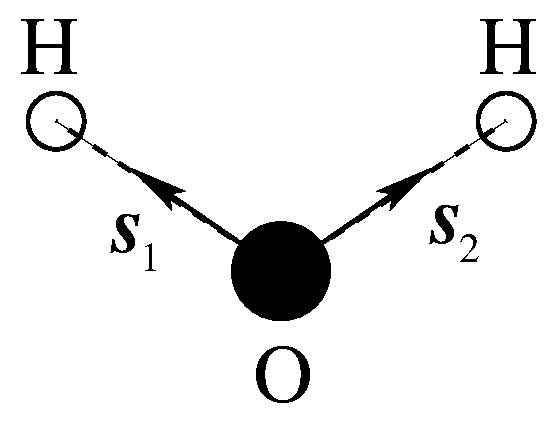
\includegraphics[width=0.2\textwidth]{fig/water.eps}
  \caption{A schematic plot of three-point-charge rigid water molecule.
  Its orientation is defined by vectors $\vect s_1$ and $\vect s_2$.}
  \label{fig:tmp1}
\end{figure}

We now calculate the single molecular partition funtion in the momenta space:
\begin{align}
  q(V,T) =
  \int \dd\vect p_1\dd\vect p_2\dd\vect p_3
  \prod_{\alpha=1}^3
  \delta (C_p^\alpha (\vect p_1,\vect p_2,\vect p_3))
  e^{-\beta (\frac{\vect p_1^2}{2 m_1} + \frac{\vect p_2^2}{2 m_2} + \frac{\vect p_3^2}{2 m_3})}
\end{align}
Convert all momenta to velocity yields,
\begin{align}
  q(V,T) =
  m^3_1 m^3_2 m^3_3 \int \dd\vect v_1\dd\vect v_2\dd\vect v_3
  \prod_{\alpha=1}^3
  \delta (C_p^\alpha (m_1\vect v_1,m_2\vect v_2,m_3\vect v_3))
  e^{-\beta (\frac12m_1\vect v_1^2 + \frac12m_2\vect v_2^2 + \frac12m_3\vect v_3^2)}
\end{align}
Without lost of generality, we assume 1 and 2 are hydrogen atoms, and 3 is an oxygen atoms. The corresponding masses are $m_H$ and $m_O$.
We assume the configuration of the water is given by two unit vectors $\vect s_1$ and
$\vect s_2$, see Fig~\ref{fig:tmp1}. Note that they are no
now, we can explicitly write down the constraints for the momenta:
\begin{align}
  C_p^1 (m_1\vect v_1,m_2\vect v_2,m_3\vect v_3)
  &= \vect v_1\cdot\vect s_1 - \vect v_3\cdot\vect s_1\\
  C_p^2 (m_1\vect v_1,m_2\vect v_2,m_3\vect v_3)
  &= \vect v_2\cdot\vect s_2 - \vect v_3\cdot\vect s_2\\
  C_p^3 (m_1\vect v_1,m_2\vect v_2,m_3\vect v_3)
  &= (\vect v_1 - \vect v_2)\cdot(\vect s_1 - \vect s_2)
\end{align}
It would be convenient if we present $\vect v_1$ and $\vect v_2$
by the relative velocities with respect to $\vect v_3$:
$\vect v_1 = \vect v_1 - \vect v_3$ and 
$\vect v_2 = \vect v_2 - \vect v_3$. We have
\begin{align}
  q(V,T) =
  m_H^6m_O^3
  \int \dd\vect v_3
  e^{-\beta \frac12m_O\vect v_3^2}
  \int \dd\vect v_1\dd\vect v_2
  \delta(\vect v_1\cdot\vect s_1)
  \delta(\vect v_2\cdot\vect s_2)
  \delta((\vect v_1 - \vect v_2)\cdot(\vect s_1 - \vect s_2))
  e^{-\beta (\frac12m_H\vect v_1^2 + \frac12m_H\vect v_2^2)}
\end{align}
By presenting $\vect s_1$, $\vect s_2$,
$\vect v_1$ and $\vect v_2$ in the local coordinate
defined by $\vect e_1, \vect e_2, \vect e_3 = \vect e_1\times\vect e_2$
(see Fig~\ref{fig:tmp1}), we define
\begin{align}
\vect s_1 &= s_1\vect e_1 + s_2\vect e_2  \\
\vect s_2 &= -s_1\vect e_1 + s_2\vect e_2    
\end{align}
by considering the constraints, we have
\begin{align}
\vect v_1 &= v_1\vect e_1 - \frac{s_1}{s_2}v_1\vect e_2 + w_1\vect e_3\\
\vect v_2 &= v_1\vect e_1 + \frac{s_1}{s_2}v_1\vect e_2 + w_2\vect e_3
\end{align}
The Leimann measure of the submanifold reads:
\begin{align}
  g = \sqrt{
    \bigg(
    \frac{\partial(\vect v_1, \vect v_2)}
    {\partial(v_1,w_1,w_2)}
    \bigg)^T
    \cdot
    \bigg(
    \frac{\partial(\vect v_1, \vect v_2)}
    {\partial(v_1,w_1,w_2)}
    \bigg)
  }
  = \sqrt 2 \;\nu
\end{align}
We denote $\nu^2 = (s_1^2 + s_2^2) / s_2^2$.
The partition function writes,
\begin{align}
  q(V,T) =
  \frac{h^\frac32}{m_H^3}
  m_H^6 m_O^3
  \int \dd\vect v_3
  e^{-\beta \frac12m_O\vect v_3^2}
  \int \dd v_1\dd w_1\dd w_2\:g\cdot
  e^{-\beta (m_H\nu^2 v_1^2 + \frac12m_H w_1^2 + \frac12m_H w_2^2)}
\end{align}
The prefector ${h^\frac32}/{m_H^3}$ comes from the Heissenberg's principle
of uncertainty: $\dd r\dd p = h$, and here we
heuristically denote $\dd p = \sqrt h$, or
$\dd v  = \sqrt h/m$.
By calculating the integral by hand, we have 
\begin{align}
  q(V,T) &=
  \frac{h^\frac32}{m_H^3}
  m_H^6 m_O^3
  \sqrt 2\,\nu\,
  \sqrt{
    \bigg(
    \frac{2\pi k_BT}{m_O}
    \bigg)^3
  }
  \cdot
  \sqrt{
    \frac{2\pi k_BT}{2\nu^2m_H}
  }
  \cdot
  \sqrt{
    \bigg(
    \frac{2\pi k_BT}{m_H}
    \bigg)^2
  }\\
  &=
  {h^\frac32}
  \sqrt{
    (2\pi m_Hk_BT)^3
    (2\pi m_Ok_BT)^3
  }
\end{align}
  % \sqrt{2\pi m_1 k_BT}
  % \sqrt{2\pi m_2 k_BT}
  % \sqrt{2\pi (m_1 + m_2) k_BT}
The chemical potential is
\begin{align}\nonumber
  \mu 
  \approx\,&
  -\frac13 k_BT \ln
  \bigg[
  \frac{Z(3N+3,V,T)}{Z(N,V,T)}
  \bigg] \\ \nonumber
  =\,&
  -\frac13k_BT \ln
  \bigg[
  \frac{1}{N h^9}\,
  {h^{\frac32}}
  \sqrt{m_H^3m_O^3 (2\pi k_BT)^6}\\\label{eqn:mu-water-tmp1}
  &\times
  \int_{\vect C^N_r(\vect r_{3N+1}\,\vect r_{3N+2}\,\vect r_{3N+3})=0}\dd\vect r_{3N+1}\,\dd\vect r_{3N+2}\,\dd\vect r_{3N+3}
  \Big\langle e^{-\beta\Delta U} \Big\rangle_{\vect r_1, \cdots,\vect r_{3N}}
  \bigg]
  % \\ \nonumber  
  % =\,&
  % -k_BT \ln
  % \bigg[
  % \frac{V^3}{N h^6 \vert \nu\vert}
  % \sqrt{m_1 m_2 (m_1+m_2) m_3^3 (2\pi k_BT)^6}\\\nonumber
  % &\times
  % \int\dd\vect r_{3N+1}\,\dd\vect r_{3N+2}\,\dd\vect r_{3N+3}
  % \frac{1}{V^3}
  % \prod_{\alpha=1}^3
  % \delta(D_\alpha(\vect r_{3N+1}\,\vect r_{3N+2}\,\vect r_{3N+3}))
  % \Big\langle e^{-\beta\Delta U} \Big\rangle_{\vect r_1, \cdots,\vect r_{3N}}
  % \bigg] \\ \nonumber  
\end{align}
Now, we want to simplify the configurational partitioan function, i.e.
the integral in the Eq.~\eqref{eqn:mu-water-tmp1}.
It is more convenient to consider the relative position:
$\vect r_{3N+1} = \vect r_{3N+1}  - \vect r_{3N+3}$ and
$\vect r_{3N+2} = \vect r_{3N+2}  - \vect r_{3N+3}$, and the form
of the integral in Eq.~\eqref{eqn:mu-water-tmp1} does not change.
Since the extra chemical potential is calculated by the uniform
sampling of the hyper-isosurface defined by the constrains 
$\vect C^N_r(\vect r_{3N+1}\,\vect r_{3N+2}\,\vect r_{3N+3})=0$, the
measure of which is therefore needed:
$V\cdot 4\pi r_{OH}^2\cdot 2\pi r_{OH}\sin(\phi_{HOH}) h^\frac32$.
Therefore,
\begin{align}
  \mu
  \approx &\,
  -\frac13k_BT \ln
  \bigg[
  \frac{8\pi^2 r_{OH}^3 V \sin(\phi_{HOH})}{N h^6}
  \sqrt{m_H^3m_O^3 (2\pi k_BT)^6}
  \bigg]
  -\frac13 k_BT \ln
  \bigg[
  \Big\langle
  e^{-\beta\Delta U}
  \Big\rangle_{\vect r_1, \cdots,\vect r_{3N}}^{\vect r_{3N+1},\cdots, \vect r_{3N+3}}
  \bigg]
\end{align}
where $\big\langle
e^{-\beta\Delta U}
\big\rangle_{\vect r_1, \cdots,\vect r_{3N}}^{\vect r_{3N+1},\cdots, \vect r_{3N+3}}
$ mean the ensemble average with respect to the randomly
posited and oriented $(N+1)$-th water molecule and canonically distributed
$1,2, \cdots, N$-th water molecules.
\vskip .5cm
\noindent
To calculate the kinetic part, we have:
\begin{align}
  \mu^\kin =&\,
  -k_BT \ln
  \bigg[
  \frac{8\pi^2 r_{OH}^3 N}{V}
  \Big[\frac{m_1 m_2 (m_1+m_2)}{ (m_1 + m_2 + m_3)^3}\Big]^{\frac12}
  \bigg]
  -2k_BT \ln
  \bigg[
  \frac{V}{N}
  \Big(
  \frac{2\pi (m_1+m_2+m_3)k_BT}{h^2}
  \Big)^{\frac{3}{2}}
  \bigg] \\
  =&\,
  -k_BT \ln
  \bigg[
  \frac{8\pi^2 r_{OH}^3 N}{V}
  \Big[\frac{m_1 m_2 (m_1+m_2)}{ (m_1 + m_2 + m_3)^3}\Big]^{\frac12}
  \bigg]
  + 2 \mu_{\textrm{id}}
\end{align}
where $\mu_{\textrm{id}}$ is the chemical potential for the spherical
ideal gas.
For room temperature liquid water system,
$\mu_{\textrm{id}} = -19.3\,\textsf{kJ/mol}$,
$\mu^\kin = -19.3\times 2 + 7.6 = -31.0\,\textsf{kJ/mol}$.


\end{document}





